\documentclass[../main.tex]{subfiles}

\pagestyle{main}
\renewcommand{\chaptermark}[1]{\markboth{\chaptername\ \thechapter: #1}{}}
\setcounter{chapter}{2}

\begin{document}




\chapter{Linear Maps}
\section{The Vector Space of Linear Maps}
\begin{itemize}
    \item \marginnote{9/5:}\textbf{Linear map} (from $V$ to $W$): A function $T:V\to W$ with the following properties. \emph{Also known as} \textbf{linear transformation}.
    \begin{description}
        \item[additivity]\hfill\\ $T(u+v)=Tu+Tv$ for all $u,v\in V$.
        \item[homogeneity]\hfill\\ $T(\lambda v)=\lambda(Tv)$ for all $\lambda\in\F$ and all $v\in V$. 
    \end{description}
    \begin{itemize}
        \item Note that for linear maps, $Tv$ means the same as the more standard functional notation $T(v)$.
    \end{itemize}
    \item $\bm{\lin{V}{W}}$: The set of all linear maps from $V$ to $W$.
    \item \textbf{Zero map}: The function $0\in\lin{V}{W}$ that takes each element of some vector space to the additive identity of another vector space. \emph{Defined by}
    \begin{equation*}
        0v = 0
    \end{equation*}
    \item \textbf{Identity map}: The function $I\in\lin{V}{V}$ on some vector space that takes each element to itself. \emph{Defined by}
    \begin{equation*}
        Iv = v
    \end{equation*}
    \item We can also formalize more esoteric linear processes as linear maps.
    \begin{itemize}
        \item For example, $D\in\lin{\mathcal{P}(\R)}{\mathcal{P}(\R)}$ can be thought of as the differentiation map $Dp=p'$. This formalizes the fact that $(f+g)'=f'+g'$ and $(\lambda f)'=\lambda f'$.
        \item We can do the same with integration: Let $T\in\lin{\mathcal{P}(\R)}{\R}$ be described by $Tp=\int_0^1p(x)\dd{x}$. This formalizes the fact that integrals are additive and homogenous.
        \item \textcite{bib:Axler} gives a number more examples.
    \end{itemize}
    \item We now prove that there exists a unique linear map from a vector space of dimension $n$ to any $n$ vectors in another vector space.
    \begin{theorem}\label{trm:mapBasisToBasis}
        Suppose $v_1,\dots,v_n$ is a basis of $V$ and $w_1,\dots,w_n\in W$. Then there exists a unique linear map $T:V\to W$ such that $Tv_j=w_j$ for each $j=1,\dots,n$.
        \begin{proof}
            First, we define a function $T:V\to W$. We then show that $T$ satisfies the specified property. After that, we show that it is a linear map. Lastly, we show that it is unique. Let's begin.\par
            Let $T:V\to W$ be defined by
            \begin{equation*}
                T(c_1v_1+\cdots+c_nv_n) = c_1w_1+\cdots+c_nw_n
            \end{equation*}
            for all $c_1v_1+\cdots+c_nv_n\in V$. Note that this definition is valid since, by Theorem \ref{trm:basisLinearCombination}, each $v\in V$ can be written in the form $c_1v_1+\cdots+c_nv_n$ where $c_1,\dots,c_n\in\F$.\par
            To prove that $Tv_j=w_j$ for all $j=1,\dots,n$, let each $c_i$ in the above definition equal 0 save $c_j$, which we set equal to 1. Then we have
            \begin{align*}
                T(0v_1+\cdots+0v_{j-1}+1v_j+0v_{j+1}+\cdots+0v_n) &= 0w_1+\cdots+0w_{j-1}+1w_j+0w_{j+1}+\cdots+0w_n\\
                T(v_j) &= w_j
            \end{align*}
            as desired.\par
            To prove that $T$ is a linear map, it will suffice to verify additivity and homogeneity, which we may do as follows. Let $u,v\in V$ with $u=a_1v_1+\cdots+a_nv_n$ and $v=c_1v_1+\cdots+c_nv_n$, and let $\lambda\in\F$. Then
            \begin{align*}
                T(u+v) &= T((a_1+c_1)v_1+\cdots+(a_n+c_n)v_n)\\
                &= (a_1+c_1)w_1+\cdots+(a_n+c_n)w_n\\
                &= Tu+Tv
            \end{align*}
            and
            \begin{align*}
                T(\lambda v) &= T(\lambda c_1v_1+\cdots+\lambda c_nv_n)\\
                &= \lambda c_1w_1+\cdots+\lambda c_nw_n\\
                &= \lambda Tv
            \end{align*}
            as desired.\par
            Now suppose $\tilde{T}\in\lin{V}{W}$ satisfies $\tilde{T}v_j=w_j$ for all $j=1,\dots,n$. To prove that $T=\tilde{T}$, it will suffice to show that $\tilde{T}(c_1v_1+\cdots+c_nv_n)=T(c_1v_1+\cdots+c_nv_n)$ for all $c_1v_1+\cdots+c_nv_n\in V$. Let $c_1v_1+\cdots+c_nv_n\in V$ be arbitrary. We know that $\tilde{T}(v_j)=w_j$ for all $j=1,\dots,n$. It follows since $\tilde{T}$ is a linear map (specifically, since it's homogenous) that $c_jw_j=c_j\tilde{T}(v_j)=\tilde{T}(c_jv_j)$ for all $j=1,\dots,n$. Similarly, the additivity of $\tilde{T}$ implies that
            \begin{align*}
                T(c_1v_1+\cdots+c_nv_n) &= c_1w_1+\cdots+c_nw_n\\
                &= \tilde{T}(c_1v_1)+\cdots+\tilde{T}(c_nv_n)\\
                &= \tilde{T}(c_1v_1+\cdots+c_nv_n)
            \end{align*}
            as desired.
        \end{proof}
    \end{theorem}
    \item \textbf{Sum} (of $S,T\in\lin{V}{W}$): The linear map $(S+T)\in\lin{V}{W}$ defined by $(S+T)(v)=Sv+Tv$ for all $v\in V$.
    \item \textbf{Product} (of $T\in\lin{V}{W}$ and $\lambda\in\F$): The linear map $(\lambda T)\in\lin{V}{W}$ defined by $(\lambda T)(v)=\lambda(Tv)$ for all $v\in V$.
    \item It follows that, under these definitions of addition and multiplication, $\lin{V}{W}$ is a vector space.
    \item \textbf{Product} (of $T\in\lin{U}{V}$ and $S\in\lin{V}{W}$): The linear map $ST\in\lin{U}{W}$ defined by $(ST)(u)=S(Tu)$ for all $u\in U$.
    \begin{itemize}
        \item Note that the product is just function composition, but most mathematicians do write $ST$ instead of $S\circ T$.
    \end{itemize}
    \item Linear maps (with the correct corresponding domains) satisfy the associativity, identity, and distributive properties. However, multiplication of linear maps is not necessarily commutative.
    \begin{itemize}
        \item $(T_1T_2)T_3=T_1(T_2T_3)$.
        \item $TI_V=I_WT=T$ (note that if $T\in\lin{V}{W}$, $I_V\in\lin{V}{V}$ and $I_W\in\lin{W}{W}$).
        \item $(S_1+S_2)T=S_1T+S_2T$ and $S(T_1+T_2)=ST_1+ST_2$.
    \end{itemize}
    \item Linear maps send 0 to 0.
    \begin{theorem}\label{trm:linSendsZero}
        Suppose $T\in\lin{V}{W}$. Then $T(0)=0$.
        \begin{proof}
            By additivity, we have
            \begin{align*}
                T(0) &= T(0+0) = T(0)+T(0)\\
                0 &= T(0)
            \end{align*}
            as desired.
        \end{proof}
    \end{theorem}
\end{itemize}



\section{Null Spaces and Ranges}
\begin{itemize}
    \item \textbf{Null space} (of $T\in\lin{V}{W}$): The subset of $V$ consisting of those vectors that $T$ maps to 0. \emph{Also known as} \textbf{kernel}. \emph{Denoted by} $\bm{\nul T}$. \emph{Given by}
    \begin{equation*}
        \nul T = \{v\in V:Tv=0\}
    \end{equation*}
    \item The null space is a subspace.
    \begin{theorem}\label{trm:nullSpace}
        Suppose $T\in\lin{V}{W}$. Then $\nul T$ is a subspace of $V$.
        \begin{proof}
            To prove that $\nul T$ is a subspace of $V$, it will suffice to show that $0\in\nul T$, $u,v\in\nul T$ implies that $u+v\in\nul T$, and $u\in\nul T$ and $\lambda\in\F$ imply $\lambda u\in\nul T$. Let's begin.\par
            By Theorem \ref{trm:linSendsZero}, $T(0)=0$. Therefore, $0\in\nul T$, as desired.\par
            Let $u,v\in\nul T$ be arbitrary. Then by additivity
            \begin{equation*}
                T(u+v) = Tu+Tv = 0+0 = 0
            \end{equation*}
            so $u+v\in\nul T$, as desired.\par
            Let $u\in\nul T$ and $\lambda\in\F$ be arbitrary. Then by homogeneity,
            \begin{equation*}
                T(\lambda u) = \lambda Tu = \lambda 0 = 0
            \end{equation*}
            so $\lambda u\in\nul T$, as desired.
        \end{proof}
    \end{theorem}
    \item \textbf{Injective} (function): A function $T:V\to W$ such that $Tu=Tv$ implies $u=v$. \emph{Also known as} \textbf{one-to-one}.
    \item If 0 is the only vector that gets mapped to 0, then $T$ is injective.
    \begin{theorem}\label{trm:nullSpaceInjective}
        Let $T\in\lin{V}{W}$. Then $T$ is injective if and only if $\nul T=\{0\}$.
        \begin{proof}
            Suppose first that $T$ is injective. To prove that $\nul T=\{0\}$, it will suffice to show that $0\in\nul T$ and for every $v\in\nul T$, $v=0$. By Theorem \ref{trm:nullSpace}, $0\in\nul T$. Now let $v\in\nul T$ be arbitrary. By the definition of the null space, we have $Tv=0$. By Theorem \ref{trm:linSendsZero}, we have $T(0)=0$. Thus, by transitivity, we have that $Tv=T(0)$. It follows by injectivity that $v=0$, as desired.\par
            Now suppose that $\nul T=\{0\}$. To prove that $T$ is injective, it will suffice to show that if $Tu=Tv$, then $u=v$. Suppose $u,v\in V$ satisfy $Tu=Tv$. Then
            \begin{equation*}
                0 = Tu-Tv = T(u-v)
            \end{equation*}
            so $(u-v)\in\nul T=\{0\}$. It follows that $u-v=0$, i.e., that $u=v$, as desired.
        \end{proof}
    \end{theorem}
    \item \textbf{Range} (of $T\in\lin{V}{W}$): The subset of $W$ consisting of those vectors that are of the form $Tv$ for some $v\in V$. \emph{Also known as} \textbf{image}. \emph{Denoted by} $\bm{\range T}$. \emph{Given by}
    \begin{equation*}
        \range T = \{Tv:v\in V\}
    \end{equation*}
    \item The range is a subspace.
    \begin{theorem}\label{trm:rangeSpace}
        Suppose $T\in\lin{V}{W}$. Then $\range T$ is a subspace of $W$.
        \begin{proof}
            To prove that $\range T$ is a subspace of $W$, it will suffice to show that $0\in\range T$, $w_1,w_2\in\range T$ implies that $(w_1+w_2)\in\range T$, and $w\in\range T$ and $\lambda\in\F$ imply $\lambda w\in\range T$. Let's begin.\par
            By the definition of a vector space, $0\in V$. By Theorem \ref{trm:linSendsZero}, $T(0)=0$. Therefore, $0\in\range T$, as desired.\par
            Let $w_1,w_2\in\range T$ be arbitrary. Then there exist $v_1,v_2\in V$ such that $Tv_1=w_1$ and $Tv_2=w_2$. It follows by additivity that
            \begin{equation*}
                T(v_1+v_2) = Tv_1+Tv_2 = w_1+w_2
            \end{equation*}
            Therefore, since $v_1+v_2\in V$, we have that $(w_1+w_2)\in\range T$, as desired.\par
            Let $w\in\range T$ and $\lambda\in\F$ be arbitrary. Then there exists $v\in V$ such that $Tv=w$. It follows by homogeneity that
            \begin{equation*}
                T(\lambda v) = \lambda Tv = \lambda w
            \end{equation*}
            Therefore, since $\lambda v\in V$, we have that $\lambda w\in\range T$, as desired.
        \end{proof}
    \end{theorem}
    \item \textbf{Surjective} (function): A function $T:V\to W$ such that $\range T=W$. \emph{Also known as} \textbf{onto}.
    \item We now prove a very important theorem.
    \begin{theorem}[Fundamental Theorem of Linear Maps]\label{trm:fundamentalTheoremLinearMaps}
        Suppose $V$ is finite-dimensional and $T\in\lin{V}{W}$. Then $\range T$ is finite-dimensional and
        \begin{equation*}
            \dim V = \dim\nul T+\dim\range T
        \end{equation*}
        \begin{proof}
            By Theorem \ref{trm:nullSpace}, $\nul T$ is a subspace of $V$ finite-dimensional. Thus, by Theorem \ref{trm:finiteDimensionalSubspaces}, $\nul T$ is finite-dimensional. It follows by Theorem \ref{trm:finiteBasis} that we may let $u_1,\dots,u_m$ be a basis of $\nul T$. As a basis of a subspace of $V$, $u_1,\dots,u_m$ is a linearly independent list of vectors in $V$. Consequently, by Theorem \ref{trm:lnlIndependentExtendBasis}, we may extend it to a basis $u_1,\dots,u_m,v_1,\dots,v_n$ of $V$.\par
            Having established this terminology, we can now see that to prove that $\range T$ is finite-dimensional, it will suffice to show that $Tv_1,\dots,Tv_n$ spans it. To show that $\spn(Tv_1,\dots,Tv_n)=\range T$, it will suffice to show that every $b_1Tv_1+\cdots+b_nTv_n\in\spn(Tv_1,\dots,Tv_n)$ is an element of $\range T$ and that every $Tv\in\range T$ is an element of $\spn(Tv_1,\dots,Tv_n)$. Let $b_1Tv_1+\cdots+b_nTv_n\in\spn(Tv_1,\dots,Tv_n)$ be arbitrary. Then
            \begin{align*}
                b_1Tv_1+\cdots+b_nTv_n &= T(b_1v_1+\cdots+b_nv_n)\\
                &= T(0u_1+\cdots+0u_m+b_1v_1+\cdots+b_nv_n)
            \end{align*}
            Therefore, since $0u_1+\cdots+0u_m+b_1v_1+\cdots+b_nv_n\in V$ by $V$'s closure under addition and scalar multiplication, we have that $b_1Tv_1+\cdots+b_nTv_n\in\range T$, as desired. Now let $Tv\in\range T$ be arbitrary. Since $v\in V$ and $u_1,\dots,u_m,v_1,\dots,v_n$ is a basis of $V$, Theorem \ref{trm:basisLinearCombination} implies that $v=a_1u_1+\cdots+a_mu_m+b_1v_1+\cdots+b_nv_n$ for some $a_1,\dots,a_m,b_1,\dots,b_n\in\F$. Therefore,
            \begin{align*}
                Tv &= T(a_1u_1+\cdots+a_mu_m+b_1v_1+\cdots+b_nv_n)\\
                &= T(a_1u_1+\cdots+a_mu_m)+T(b_1v_1+\cdots+b_nv_n)\\
                &= a_1Tu_1+\cdots+a_mTu_m+b_1Tv_1+\cdots+v_nTv_n\\
                &= a_10+\cdots+a_m0+b_1Tv_1+\cdots+v_nTv_n\\
                &= b_1Tv_1+\cdots+v_nTv_n
            \end{align*}
            where each $Tu_j=0$ because each $u_j\in\nul T$, so $Tv\in\spn(Tv_1,\dots,Tv_n)$, as desired.\par
            Before we can verify the equation from the theorem, we need to establish one last fact: that $Tv_1,\dots,Tv_n$ is linearly independent. Suppose $c_1,\dots,c_n\in\F$ make
            \begin{align*}
                c_1Tv_1+\cdots+c_nTv_n &= 0\\
                T(c_1v_1+\cdots+c_nv_n) &= 0
            \end{align*}
            It follows that $c_1v_1+\cdots+c_nv_n\in\nul T$. Thus, since $u_1,\dots,u_m$ is a basis of $\nul T$ by Theorem \ref{trm:basisLinearCombination}, we have that
            \begin{align*}
                c_1v_1+\cdots+c_nv_n &= d_1u_1+\cdots+d_mu_m\\
                0 &= d_1u_1+\cdots+d_mu_m-c_1v_1-\cdots-c_nv_n
            \end{align*}
            for some $d_1,\dots,d_m\in\F$. But since $u_1,\dots,u_m,v_1,\dots,v_n$ is linearly independent as the basis of $V$, the above equation implies that $c_1=\cdots=c_n=0$, as desired.\par
            Having established that $u_1,\dots,u_m,v_1,\dots,v_n$ is a basis of $V$, $u_1,\dots,u_m$ is a basis of $\nul T$, and $Tv_1,\dots,Tv_n$ spans $\range T$ and is linearly independent in $\range T$ (i.e., is a basis of $\range T$), we have that
            \begin{align*}
                \dim V &= m+n\\
                &= \dim\nul T+\dim\range T
            \end{align*}
            as desired.
        \end{proof}
    \end{theorem}
    \item We can now prove that a linear map to a "smaller" vector space cannot be injective.
    \begin{theorem}\label{trm:smallerNotInjective}
        Suppose $V$ and $W$ are finite-dimensional vector spaces such that $\dim V>\dim W$. Then no linear map from $V$ to $W$ is injective.
        \begin{proof}
            Let $T\in\lin{V}{W}$. Then
            \begin{align*}
                \dim\nul T &= \dim V-\dim\range T\tag*{\hyperref[trm:fundamentalTheoremLinearMaps]{Fundamental Theorem of Linear Maps}}\\
                &\geq \dim V-\dim\range T\tag*{Theorem \ref{trm:dimSubspaces}}\\
                &> 0
            \end{align*}
            It follows that $\nul T$ has a basis consisting of a list of one or more vectors. As a linearly independent list, naturally none of these vectors will be equal to the zero vector. Thus, since $\nul T$ contains vectors other than 0, Theorem \ref{trm:nullSpaceInjective} implies that $T$ is not injective.
        \end{proof}
    \end{theorem}
    \item Similarly, we can prove that a linear map to a "bigger" vector space cannot be surjective.
    \begin{theorem}\label{trm:biggerNotSurjective}
        Suppose $V$ and $W$ are finite-dimensional vector spaces such that $\dim V<\dim W$. Then no linear map from $V$ to $W$ is surjective.
        \begin{proof}
            Let $T\in\lin{V}{W}$. Then
            \begin{align*}
                \dim\range T &= \dim V-\dim\nul T\tag*{\hyperref[trm:fundamentalTheoremLinearMaps]{Fundamental Theorem of Linear Maps}}\\
                &\leq \dim V
                &< \dim W
            \end{align*}
            Therefore, $\range T\neq W$, so $T$ cannot be surjective.
        \end{proof}
    \end{theorem}
    \item Theorems \ref{trm:smallerNotInjective} and \ref{trm:biggerNotSurjective} allow us to express questions about systems of linear equations in terms of linear maps.
    \begin{itemize}
        \item For example, a question about a \textbf{homogenous} system of linear equations could be, "does there exist a nonzero solution to the homogenous system $\sum_{k=1}^nA_{1,k}x_k=0,\dots,\sum_{k=1}^nA_{m,k}x_k=0$?"
        \item If we define $T:\F^n\to\F^m$ by
        \begin{equation*}
            T(x_1,\dots,x_n) = \left( \sum_{k=1}^nA_{1,k}x_k,\dots,\sum_{k=1}^nA_{m,k}x_k \right)
        \end{equation*}
        we can express the system of equations as $T(x_1,\dots,x_n)=0$ and ask instead, "is $\dim\nul T>0$?"
    \end{itemize}
    \item \textbf{Homogenous} (system of linear equations): A system of $m$ linear equations $\sum_{k=1}^nA_{1,k}x_k=c_1$ through $\sum_{k=1}^nA_{m,k}x_k=c_m$ such that the constant term $c_j=0$ for all $j=1,\dots,m$.
    \item Continuing with the linear equations example, we can rigorously show the following.
    \begin{theorem}
        A homogenous system of linear equations with more variables than equations has nonzero solutions.
        \begin{proof}
            In terms of the above, $T:\F^n\to\F^m$ where $n>m$. Thus, by Theorem \ref{trm:smallerNotInjective}, $T$ is not injective. Consequently, by Theorem \ref{trm:nullSpaceInjective}, $\dim\nul T>0$. Therefore, the system has nonzero solutions.
        \end{proof}
    \end{theorem}
    \begin{theorem}
        An inhomogenous system of linear equations with more equations than variables has no solution for some choice of constant terms.
        \begin{proof}
            In terms of the above, $T:\F^n\to\F^m$ where $m>n$. We want to know if there exists $(c_1,\dots,c_m)\in\F^m$ such that $T(x_1,\dots,x_n)\neq(c_1,\dots,c_m)$ for any $(x_1,\dots,x_n)\in\F^n$. In other words, we want to know if there exists $(c_1,\dots,c_m)\in\F^m$ such that $(c_1,\dots,c_m)\notin\range T$, i.e., if $\range T\neq\F^m$. But since $n<m$, Theorem \ref{trm:biggerNotSurjective} asserts that $T$ is not surjective, meaning that $\range T\neq W$, as desired.
        \end{proof}
    \end{theorem}
    \begin{itemize}
        \item Note that while the past two results are typically proven with Gaussian elimination, the abstract approach taken here leads to cleaner proofs.
    \end{itemize}
\end{itemize}



\section{Matrices}
\begin{itemize}
    \item \textbf{$\bm{m}$-by-$\bm{n}$ matrix}: A rectangular array $A$ of elements of $\F$ with $m$ rows and $n$ columns
    \begin{equation*}
        A =
        \begin{pmatrix}
            A_{1,1} & \cdots & A_{1,n}\\
            \vdots &  & \vdots\\
            A_{m,1} & \cdots & A_{m,n}\\
        \end{pmatrix}
    \end{equation*}
    where $m$ and $n$ are positive integers.
    \begin{itemize}
        \item The notation $A_{j,k}$ denotes the entry in row $j$, column $k$ of $A$. In other words, the first index refers to the row nunber and the second index refers to the column number.
    \end{itemize}
    \item \textbf{Matrix} (of $T\in\lin{V}{W}$ with respect to the bases $v_1,\dots,v_n$ of $V$ and $w_1,\dots,w_m$ of $W$): The $m$-by-$n$ matrix $\mat{T}$ whose entries $A_{j,k}$ are defined by
    \begin{equation*}
        Tv_k = A_{1,k}w_1+\cdots+A_{m,k}w_m
    \end{equation*}
    \begin{itemize}
        \item If the bases are not clear from context, then the notation $\mat{T,(v_1,\dots,v_n),(w_1,\dots,w_m)}$ is used.
        \item Another way of wording the definition states that the $k^\text{th}$ column of $\mat{T}$ consists of the scalars needed to write $Tv_k$ as a linear combination of $w_1,\dots,w_m$.
        \item Assuming standard bases, we \dq{can think of the $k^\text{th}$ column of $\mat{T}$ as the $T$ applied to the $k^\text{th}$ standard basis vector}{71}
    \end{itemize}
    \item \textbf{Sum} (of two $m$-by-$n$ matrices $A,C$): The $m$-by-$n$ matrix $A+C$ defined by $(A+C)_{j,k}=A_{j,k}+C_{j,k}$.
    \begin{itemize}
        \item Symbolically,
        \begin{equation*}
            \begin{pmatrix}
                A_{1,1} & \cdots & A_{1,n}\\
                \vdots &  & \vdots\\
                A_{m,1} & \cdots & A_{m,n}\\
            \end{pmatrix}+
            \begin{pmatrix}
                C_{1,1} & \cdots & C_{1,n}\\
                \vdots &  & \vdots\\
                C_{m,1} & \cdots & C_{m,n}\\
            \end{pmatrix}
            =
            \begin{pmatrix}
                A_{1,1}+C_{1,1} & \cdots & A_{1,n}+C_{1,n}\\
                \vdots &  & \vdots\\
                A_{m,1}+C_{m,1} & \cdots & A_{m,n}+C_{m,n}\\
            \end{pmatrix}
        \end{equation*}
    \end{itemize}
    \item Suppose $S,T\in\lin{V}{W}$. Then $\mat{S+T}=\mat{S}+\mat{T}$.
    \item \textbf{Product} (of an $m$-by-$n$ matrix $A$ and $\lambda\in\F$): The $m$-by-$n$ matrix $\lambda A$ defined by $(\lambda A)_{j,k}=\lambda A_{j,k}$.
    \begin{itemize}
        \item Symbolically,
        \begin{equation*}
            \lambda
            \begin{pmatrix}
                A_{1,1} & \cdots & A_{1,n}\\
                \vdots &  & \vdots\\
                A_{m,1} & \cdots & A_{m,n}\\
            \end{pmatrix}
            =
            \begin{pmatrix}
                \lambda A_{1,1} & \cdots & \lambda A_{1,n}\\
                \vdots &  & \vdots\\
                \lambda A_{m,1} & \cdots & \lambda A_{m,n}\\
            \end{pmatrix}
        \end{equation*}
    \end{itemize}
    \item Suppose $\lambda\in\F$ and $T\in\lin{V}{W}$. Then $\mat{\lambda T}=\lambda\mat{T}$.
    \item $\protect\fakebold{\F}^{\bm{m,n}}$: The set of all $m$-by-$n$ matrices with entries in $\F$, where $m$ and $n$ are positive integers.
    \item We have that $\dim\F^{m,n}=mn$.
    \begin{itemize}
        \item Note that a basis of $\F^{m,n}$ is the set of all $m$-by-$n$ matrices that have 0s everywhere save a 1 in a single place.
    \end{itemize}
    \item \textbf{Product} (of an $m$-by-$n$ matrix $A$ and an $n$-by-$p$ matrix $C$): The $m$-by-$p$ matrix $AC$ defined by $(AC)_{j,k}=\sum_{r=1}^nA_{j,r}C_{r,k}$.
    \begin{itemize}
        \item We may derive this by noting that if $\mat{S}=A$ and $\mat{T}=C$, $T:U\to V$ and $S:V\to W$, and $u_1,\dots,u_p$, $v_1,\dots,v_n$, and $w_1,\dots,w_m$ are bases, then
        \begin{align*}
            (ST)u_k &= S\left( \sum_{r=1}^nC_{r,k}v_r \right)\\
            &= \sum_{r=1}^nC_{r,k}Sv_r\\
            &= \sum_{r=1}^nC_{r,k}\sum_{j=1}^mA_{j,r}w_j\\
            &= \sum_{j=1}^m\left( \sum_{r=1}^nA_{j,r}C_{r,k} \right)w_j
        \end{align*}
        \item Matrix multiplication is not commutative, but is distributive and associative.
    \end{itemize}
    \item We now prove a relation between matrix and operator composition.
    \begin{theorem}\label{trm:matSTmatSmatT}
        Suppose $T\in\lin{U}{V}$ and $S\in\lin{V}{W}$. Then $\mat{ST}=\mat{S}\mat{T}$.
    \end{theorem}
    \item If $A$ is an $m$-by-$n$ matrix, then\dots
    \begin{itemize}
        \item We let $A_{j,\cdot}$ denote the 1-by-$n$ matrix consisting of row $j$ of $A$;
        \item We let $A_{\cdot,k}$ denote the $m$-by-1 matrix consisting of column $k$ of $A$.
    \end{itemize}
    \item Thus, if $A$ is an $m$-by-$n$ matrix and $C$ is an $n$-by-$p$ matrix, then $(AC)_{j,k}=A_{j,\cdot}C_{\cdot,k}$ for all $1\leq j\leq m$ and $1\leq k\leq p$.
    \item Similarly, $(AC)_{\cdot,k}=AC_{\cdot,k}$.
    \item Lastly, suppose $A$ is an $m$-by-$n$ matrix and $c=(c_1,\dots,c_n)$ is an $n$-by-1 matrix. Then $Ac=c_1A_{\cdot,1}+\cdots+c_nA_{\cdot,n}$.
    \begin{itemize}
        \item In other words, $Ac$ is a linear combination of the columns of $A$, with the scalars that multiply the columns coming from $c$.
    \end{itemize}
\end{itemize}



\section{Invertibility and Isomorphic Vector Spaces}
\begin{itemize}
    \item \marginnote{9/6:}\textbf{Invertible} (linear map): A linear map $T\in\lin{V}{W}$ such that there exists a linear map $S\in\lin{V}{W}$ such that $ST$ equals the identity map on $V$ and $TS$ equals the identity map on $W$.
    \item \textbf{Inverse} (of $T\in\lin{V}{W}$): The linear map $S\in\lin{W}{V}$ satisfying $ST=I_V$ and $TS=I_W$. \emph{Denoted by} $\bm{T^{-1}}$.
    \item We now justify the use of the word "the" in the definition of the inverse.
    \begin{theorem}\label{trm:uniqueInverse}
        An invertible linear map has a unique inverse.
        \begin{proof}
            Suppose $T\in\lin{V}{W}$ is invertible and $S_1,S_2$ are inverses of $T$. Then
            \begin{equation*}
                S_1 = S_1I = S_1(TS_2) = (S_1T)S_2 = IS_2 = S_2
            \end{equation*}
            as desired.
        \end{proof}
    \end{theorem}
    \item We now give a criterion for invertibility.
    \begin{theorem}\label{trm:invertibleInjectiveSurjective}
        A linear map is invertible if and only if it is injective and surjective.
        \begin{proof}
            Let $T\in\lin{V}{W}$. Suppose first that $T$ is invertible.\par
            To prove that $T$ is injective, it will suffice to show that for all $u,v\in V$, $Tu=Tv$ implies that $u=v$. Let $u,v$ be arbitrary elements of $V$ that satisfy $Tu=Tv$. Then
            \begin{equation*}
                u = T^{-1}(Tu) = T^{-1}(Tv) = v
            \end{equation*}
            as desired.\par
            To prove that $T$ is surjective, it will suffice to show that $\range T=W$. Since $\range T\subset W$, we need only show that $W\subset\range T$. Let $w\in W$ be arbitrary. Since $w=T(T^{-1}w)$ where $T^{-1}w\in V$, we have that $w\in\range T$, as desired.\par\smallskip
            Now suppose that $T$ is injective and surjective. To prove that $T$ is invertible, we will define a function $S:W\to V$, prove that it is a linear map, prove that $TS=I_W$, and prove that $ST=I_V$. Let $Sw$ be the unique element of $V$ such that $T(Sw)=w$ (the surjectivity of $T$ guarantees that there exists \emph{an} element of $V$ that $T$ maps to $w$, and the injectivity of $T$ guarantees the uniqueness of said element).\par
            To prove that $S$ is a linear map, it will suffice to show that $S$ is additive and homogenous. To verify additivity, first note that the additivity of $T$ implies that
            \begin{equation*}
                T(Sw_1+Sw_2) = T(Sw_1)+T(Sw_2) = w_1+w_2
            \end{equation*}
            But since the above equation implies that $Sw_1+Sw_2$ is the unique element of $V$ that $T$ maps to $w_1+w_2$, we have by the definition of $S$ that $S(w_1+w_2)=Sw_1+Sw_2$. The proof is symmetric for homogeneity.\par
            To prove that $TS=I_W$, we need only appeal to the definition of $S$, which states that $(TS)w=T(Sw)=w$ for all $w\in W$. It immediately follows that $TS=I_W$.\par
            To prove that $ST=I_V$, first note that for all $v\in V$,
            \begin{equation*}
                T((ST)v) = (TS)(Tv) = I(Tv) = Tv
            \end{equation*}
            It follows by the injectivity of $T$ that $(ST)v=v$, i.e., that $ST=I_V$, as desired.
        \end{proof}
    \end{theorem}
    \item \textbf{Isomorphism}: An invertible linear map.
    \item \textbf{Isomorphic} (vector spaces): Two vector spaces such that there exists an isomorphism from one vector space onto the other one.
    \item Isomorphic vector spaces have the same dimension.
    \begin{theorem}\label{trm:dimIsomorphic}
        Two finite-dimensional vector spaces over $\F$ are isomorphic if and only if they have the same dimension.
        \begin{proof}
            Suppose $V,W$ are isomorphic finite-dimensional vector spaces over $\F$. Then there exists an isomorphism $T:V\to W$. By the definition of isomorphism, $T$ is an invertible linear map, meaning by Theorem \ref{trm:invertibleInjectiveSurjective} that $T$ is injective and surjective. Thus, since there exists an injective linear map $T:V\to W$, the contrapositive of Theorem \ref{trm:smallerNotInjective} asserts that $\dim V\leq\dim W$. Additionally, since there exists a surjective linear map $T:V\to W$, the contrapositive of Theorem \ref{trm:biggerNotSurjective} asserts that $\dim V\geq\dim W$. Therefore, we have that $\dim V=\dim W$, as desired.\par
            Now suppose that $\dim V=\dim W$. Let $v_1,\dots,v_n$ be a basis of $V$, and let $w_1,\dots,w_n$ be a basis of $W$. By Theorem \ref{trm:mapBasisToBasis}, there exists a unique linear map $T:V\to W$ such that $Tv_j=w_j$ for each $j=1,\dots,n$. To prove that $T$ is an isomorphism, Theorem \ref{trm:invertibleInjectiveSurjective} tells us that it will suffice to show that it is injective and surjective. To show that $T$ is surjective, it will suffice to show that $\range T=W=\spn(w_1,\dots,w_n)$. But since $Tv_j=w_j\in\range T$ for all $j=1,\dots,n$, $\range T\subset W$, and $\range T$ is a vector space (see Theorem \ref{trm:rangeSpace}), we have that $\range T=\spn(w_1,\dots,w_n)=W$, as desired. To prove that $T$ is injective, Theorem \ref{trm:nullSpaceInjective} tells us that it will suffice to show that $\nul T=\{0\}$, i.e., that $\dim\nul T=0$. But since $\dim\range T=\dim W=\dim V$, we have by the \hyperref[trm:fundamentalTheoremLinearMaps]{Fundamental Theorem of Linear Maps} that
            \begin{align*}
                \dim\nul T+\dim\range T &= \dim V\\
                &= \dim W\\
                &= \dim\range T\\
                \dim\nul T &= 0
            \end{align*}
            as desired.
        \end{proof}
    \end{theorem}
    \item This result implies that every finite-dimensional vector space of dimension $n$ is isomorphic to $\F^n$.
    \item It also allows us to formalize the link between linear maps from $V$ to $W$ and matrices in $\F^{m,n}$.
    \begin{theorem}\label{trm:mapsMatricesIsomorphic}
        Suppose $v_1,\dots,v_n$ is a basis of $V$ and $w_1,\dots,w_m$ is a basis of $W$. Then $\mathcal{M}$ is an isomorphism between $\lin{V}{W}$ and $\F^{m,n}$.
        \begin{proof}
            We have already established that $\mat{S+T}=\mat{S}+\mat{T}$ and that $\mat{\lambda T}=\lambda\mat{T}$, so we already know that $\mathcal{M}$ is a linear map. To prove that it is invertible, Theorem \ref{trm:invertibleInjectiveSurjective} tells us that it will suffice to show that $\mathcal{M}$ is injective and surjective.\par
            To show that $\mathcal{M}$ is injective, Theorem \ref{trm:nullSpaceInjective} tells us that it will suffice to verify that $\nul\mathcal{M}=\{0\}$. Let $T\in\lin{V}{W}$ be arbitrary. If $\mat{T}=0$ (0 denoting the zero matrix), then
            \begin{equation*}
                Tv_k = 0w_1+\cdots+0w_m = 0
            \end{equation*}
            for all $k=1,\dots,n$. But since $v_1,\dots,b_n$ is a basis of $V$, this implies that $T=0$ (0 denoting the zero transformation), as desired.\par
            To show that $\mathcal{M}$ is surjective, it will suffice to verify that $\range\mathcal{M}=\F^{m,n}$. Clearly $\range\mathcal{M}\subset\F^{m,n}$, so we focus on the other direction. Let $A\in\F^{m,n}$ be arbitrary. Define $T\in\lin{V}{W}$ by
            \begin{equation*}
                Tv_k = \sum_{j=1}^mA_{j,k}w_j
            \end{equation*}
            for $k=1,\dots,n$. It follows by the definition of a matrix of a linear transformation that $\mat{T}=A$, as desired.
        \end{proof}
    \end{theorem}
    \item We can now determine the dimension of the vector space of linear maps from one finite-dimensional vector space to another.
    \begin{theorem}\label{trm:dimLVW}
        Suppose $V$ and $W$ are finite-dimensional. Then $\lin{V}{W}$ is finite-dimensional and
        \begin{equation*}
            \dim\lin{V}{W} = (\dim V)(\dim W)
        \end{equation*}
        \begin{proof}
            By Theorem \ref{trm:mapsMatricesIsomorphic}, $\lin{V}{W}$ and $\F^{m,n}$ are isomorphic. Thus, by Theorem \ref{trm:dimIsomorphic}, $\lin{V}{W}$ and $\F^{m,n}$ have the same dimension. Therefore, we have that
            \begin{align*}
                \dim\lin{V}{W} &= \dim\F^{m,n}\\
                &= mn\\
                &= (\dim V)(\dim W)
            \end{align*}
            as desired.
        \end{proof}
    \end{theorem}
    \item \textbf{Matrix} (of $v\in V$ with respect to the basis $v_1,\dots,v_n$ of $V$): The $n$-by-1 matrix $\mat{v}$ whose entries $A_{j,1}$ are defined by
    \begin{equation*}
        v = A_{1,1}v_1+\cdots+A_{n,1}v_n
    \end{equation*}
    \item We now show that the columns of the matrix of $T$ are directly related to the effect $T$ has on basis vectors.
    \begin{theorem}\label{trm:columnBasis}
        Suppose $T\in\lin{V}{W}$, $v_1,\dots,v_n$ is a basis of $V$, and $w_1,\dots,w_m$ is a basis of $W$. Let $1\leq k\leq n$. Then
        \begin{equation*}
            \mat{T}_{\cdot,k} = \mat{Tv_k}
        \end{equation*}
        \begin{proof}
            As an element of $W$, $Tv_k=c_1w_1+\cdots+c_mw_m$ for some $c_1,\dots,c_m\in\F$. By the definition of the matrix of $T$, the values in column $k$ are $c_1,\dots,c_m$. Similarly, by the definition of the matrix of $Tv_k$, the values in its one column are $c_1,\dots,c_m$, as desired.
        \end{proof}
    \end{theorem}
    \item Linear maps act like matrix multiplication.
    \begin{theorem}
        Suppose $T\in\lin{V}{W}$, $v\in V$, $v_1,\dots,v_n$ is a basis of $V$, and $w_1,\dots,w_m$ is a basis of $W$. Then
        \begin{equation*}
            \mat{Tv} = \mat{T}\mat{v}
        \end{equation*}
        \begin{proof}
            Let $v=c_1v_1+\cdots+c_nv_n$. Then by the linearity of $T$, $Tv=c_1Tv_1+\cdots+c_nTv_n$. It follows by the linearity of $\mathcal{M}$, Theorem \ref{trm:columnBasis}, and the fact that a matrix times a vector is equal to a linear combination of columns that
            \begin{align*}
                \mat{Tv} &= c_1\mat{Tv_1}+\cdots+c_n\mat{Tv_n}\\
                &= c_1\mat{T}_{\cdot,1}+\cdots+c_n\mat{T}_{\cdot,n}\\
                &= \mat{T}\mat{v}
            \end{align*}
            as desired.
        \end{proof}
    \end{theorem}
    \item \dq{Each $m$-by-$n$ matrix $A$ induces a linear map from $\F^{n,1}$ to $\F^{m,1}$, namely the matrix multiplication function that takes $x\in\F^{n,1}$ to $Ax\in\F^{m,1}$}{85}
    \item \textbf{Operator}: A linear map from a vector space to itself.
    \item $\bm{\ope{V}}$: The set of all operators on $V$.
    \begin{itemize}
        \item Mathematically, $\ope{V}=\lin{V}{V}$.
    \end{itemize}
    \item On infinite-dimensional vector spaces, neither injectivity nor surjectivity, alone, implies invertibility.
    \item However, only one does on finite-dimensional vector spaces.
    \begin{theorem}\label{trm:invertInjSurjFiniteEquivalence}
        Suppose $V$ is finite-dimensional and $T\in\ope{V}$. Then the following are equivalent.
        \begin{enumerate}[label={\textup{(}\alph*\textup{)}}]
            \item $T$ is invertible;
            \item $T$ is injective;
            \item $T$ is surjective.
        \end{enumerate}
        \begin{proof}
            First, suppose that $T$ is invertible. Then by Theorem \ref{trm:invertibleInjectiveSurjective}, $T$ is injective, as desired.\par
            Second, suppose that $T$ is injective. Then by Theorem \ref{trm:nullSpaceInjective}, $\nul T=\{0\}$. It follows by the \hyperref[trm:fundamentalTheoremLinearMaps]{Fundamental Theorem of Linear Maps} that
            \begin{align*}
                \dim\range T &= \dim V-\dim\nul T\\
                &= \dim V
            \end{align*}
            Thus, since $\range T$ has the same dimension as $V$ and is a subspace of $V$ (by Theorem \ref{trm:rangeSpace}), $\range T=V$. Therefore, $T$ is surjective, as desired.\par
            Third, suppose that $T$ is surjective. Then $\range T=V$. It follows that $\dim\range T=\dim V$. Thus, by the \hyperref[trm:fundamentalTheoremLinearMaps]{Fundamental Theorem of Linear Maps}, we have that
            \begin{align*}
                \dim\nul T &= \dim V-\dim\range T\\
                &= 0
            \end{align*}
            Consequently, by Theorem \ref{trm:nullSpaceInjective}, $T$ is injective. Therefore, by Theorem \ref{trm:invertibleInjectiveSurjective}, $T$ is invertible, as desired.
        \end{proof}
    \end{theorem}
\end{itemize}


\subsection*{Exercises}
\begin{enumerate}[label={\textbf{\arabic*}},labelsep=1em,ref={\thesection.\arabic*}]
    \setcounter{enumi}{8}
    \item \marginnote{10/11:}\label{exr:3D9}Suppose $V$ is finite-dimensional and $S,T\in\ope{V}$. Prove that $ST$ is invertible if and only if both $S$ and $T$ are invertible.
    \begin{proof}
        Suppose first that $ST$ is invertible. Then by Theorem \ref{trm:invertInjSurjFiniteEquivalence}, $ST$ is injective and surjective. We will prove that $S,T$ are invertible in turn; in particular, we will first prove that $S$ is surjective and then prove that $T$ is injective. Let's begin. To prove that $S$ is surjective, it will suffice to show that $\range S=V$. Let $v\in V$ be arbitrary. Since $ST$ is surjective, there exists $v'\in V$ such that $STv'=v$. Thus, since $Tv'\in V$, the fact that $S(Tv')=v$ implies that $v\in\range S$. The inclusion in the other direction is obvious. Now to prove that $T$ is injective, it will suffice to show that $Tv=Tv'$ implies $v'=v'$. Let $Tv=Tv'$. Then $STv=STv'$. It follows that $v=v'$ by the injectivity of $ST$, as desired.\par
        Now suppose that $S$ and $T$ are invertible. Then by Theorem \ref{trm:uniqueInverse}, there exist $S^{-1},T^{-1}$ such that
        \begin{align*}
            SS^{-1} &= I = S^{-1}S&
            TT^{-1} &= I = T^{-1}T
        \end{align*}
        Let $(ST)^{-1}=T^{-1}S^{-1}$. Then
        \begin{equation*}
            ST(ST)^{-1} = STT^{-1}S^{-1} = SIS^{-1} = SS^{-1} = I = T^{-1}T = T^{-1}IT = T^{-1}S^{-1}ST = (ST)^{-1}ST
        \end{equation*}
        so $ST$ is invertible, as desired.
    \end{proof}
    \item \label{exr:3D10}Suppose $V$ is finite-dimensional and $S,T\in\ope{V}$. Prove that $ST=I$ if and only if $TS=I$.
    \begin{proof}
        Suppose first that $ST=I$. It is easy to see that defining $(ST)^{-1}=I^{-1}=I$ yields an inverse of $ST$. Thus, since $ST$ is invertible, we have by Exercise \ref{exr:3D9} that $S$ and $T$ are invertible. It follows since $ST=I$ that $S=T^{-1}$, meaning that
        \begin{equation*}
            TS = TT^{-1} = I
        \end{equation*}
        as desired.\par
        The proof is symmetric in the other direction.
    \end{proof}
\end{enumerate}



\section{Products and Quotients of Vector Spaces}
\begin{itemize}
    \item \marginnote{9/6:}\textbf{Product} (of $V_1,\dots,V_m$): The set
    \begin{equation*}
        V_1\times\cdots\times V_m = \{(v_1,\dots,v_m):v_1\in V_1,\dots,v_m\in V_m\}
    \end{equation*}
    \begin{itemize}
        \item Addition on $V_1\times\cdots\times V_m$ is defined by
        \begin{equation*}
            (u_1,\dots,u_m)+(v_1,\dots,v_m) = (u_1+v_1,\dots,u_m+v_m)
        \end{equation*}
        \item Scalar multiplication on $V_1\times\cdots\times V_m$ is defined by
        \begin{equation*}
            \lambda(v_1,\dots,v_m) = (\lambda v_1,\dots,\lambda v_m)
        \end{equation*}
    \end{itemize}
    \item The product of $n$ vector spaces over $\F$ is a vector space over $\F$, with addition and scalar multiplication defined as above.
    \item We can, for example, identify $\R^2\times\R^3$ with $\R^5$ by constructing an isomorphism from every vector $((x_1,x_2),(x_3,x_4,x_5))\in\R^2\times\R^3$ to the vector $(x_1,x_2,x_3,x_4,x_5)\in\R^5$.
    \item The dimension of the product of vector spaces is equal to the sum of the dimensions of the component vector spaces.
    \begin{theorem}\label{trm:dimensionProduct}
        Suppose $V_1,\dots,V_m$ are finite-dimensional vector spaces. Then $V_1\times\cdots\times V_m$ is finite-dimensional and
        \begin{equation*}
            \dim(V_1\times\cdots\times V_m) = \dim V_1+\cdots+\dim V_m
        \end{equation*}
        \begin{proof}
            Choose a basis of each $V_j$. For each basis vector of each $V_j$, consider the element of $V_1\times\cdots\times V_m$ that equals the basis vector in the $j^\text{th}$ slot and 0 in the other slots. The list of all such vectors is linearly independent and spans $V_1\times\cdots\times V_m$. Thus, it is a basis of $V_1\times\cdots\times V_m$. The length of this basis is $\dim V_1+\cdots+\dim V_m$, as desired.
        \end{proof}
    \end{theorem}
    \item We now relate products and direct sums.
    \begin{theorem}\label{trm:productDirectsumInjective}
        Suppose that $U_1,\dots,U_m$ are subspaces of $V$. Define a linear map $\Gamma:U_1\times\cdots\times U_m\to U_1+\cdots+U_m$ by
        \begin{equation*}
            \Gamma(u_1,\dots,u_m) = u_1+\cdots+u_m
        \end{equation*}
        Then $U_1+\cdots+U_m$ is a direct sum if and only if $\Gamma$ is injective.
        \begin{proof}
            Suppose first that $\Gamma$ is injective. Then the only way to write 0 as a sum $u_1+\cdots+u_m$, where each $u_j\in U_j$, is by taking each $u_j=0$. It follows by the condition on direct sums that $U_1+\cdots+U_m$ is a direct sum. The proof is symmetric in the reverse direction.
        \end{proof}
    \end{theorem}
    \begin{itemize}
        \item Note that since $\Gamma$ is surjective by the definition of $U_1+\cdots+U_m$, the condition that $\Gamma$ is injective could be changed to the condition that $\Gamma$ is invertible.
    \end{itemize}
    \item We can now prove that the dimensions add up in a direct sum.
    \begin{theorem}\label{trm:dimDirectSum}
        Suppose $V$ is finite-dimensional and $U_1,\dots,U_m$ are subspaces of $V$. Then $U_1+\cdots+U_m$ is a direct sum if and only if
        \begin{equation*}
            \dim(U_1+\cdots+U_m) = \dim U_1+\cdots+\dim U_m
        \end{equation*}
        \begin{proof}
            Suppose first that $U_1+\cdots+U_m$ is a direct sum. Then by Theorem \ref{trm:productDirectsumInjective}, there exists an invertible linear map $\Gamma$ from $U_1\times\cdots\times U_m$ to $U_1+\cdots+U_m$. Thus, by Theorem \ref{trm:dimIsomorphic}, $U_1\times\cdots\times U_m$ and $U_1+\cdots+U_m$ have the same dimension. Therefore,
            \begin{align*}
                \dim(U_1+\cdots+U_m) &= \dim(U_1\times\cdots\times U_m)\\
                &= \dim U_1+\cdots+\dim U_m\tag*{Theorem \ref{trm:dimensionProduct}}
            \end{align*}
            as desired.\par
            The proof is symmetric in the other direction.
        \end{proof}
    \end{theorem}
    \item \textbf{Sum} (of $v\in V$ and $U$ a subspace of $V$): The subset of $V$ defined by
    \begin{equation*}
        v+U = \{v+u:u\in U\}
    \end{equation*}
    \item \textbf{Affine subset} (of $V$): A subset of $V$ of the form $v+U$ for some $v\in V$ and some subspace $U$ of $V$.
    \item \textbf{Parallel} (subset to $U$): An affine subset $v+U$ of $V$.
    \item \textbf{Quotient space}: The set of all affine subsets of $V$ parallel to $U$.
    \begin{figure}[H]
        \centering
        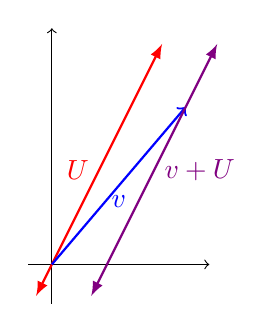
\begin{tikzpicture}
            \draw [->] (-0.3,0) -- (2,0);
            \draw [->] (0,-0.5) -- (0,3);

            \draw [red,thick,latex-latex] (-0.2,-0.4) -- node[anchor=east]{$U$} (1.4,2.8);
            \draw [blue,thick,->] (0,0) -- node[anchor=north]{$v$} (1.7,2);
            \draw [red!50!blue,thick,latex-latex] (0.5,-0.4) -- node[anchor=west]{$v+U$} (2.1,2.8);
        \end{tikzpicture}
        \caption{Visualizing $v+U$.}
        \label{fig:vU}
    \end{figure}
    \begin{itemize}
        \item Symbolically,
        \begin{equation*}
            V/U = \{v+U:v\in V\}
        \end{equation*}
    \end{itemize}
    \item Two affine subsets parallel to $U$ are equal or disjoint.
    \begin{theorem}\label{trm:affineEquivalenceProperties}
        Suppose $U$ is a subspace of $V$ and $v,w\in V$. Then the following are equivalent.
        \begin{enumerate}[label={\textup{(}\alph*\textup{)}}]
            \item $v-w\in U$;
            \item $v+U=w+U$;
            \item $(v+U)\cap(w+U)\neq\emptyset$.
        \end{enumerate}
        \begin{proof}
            First, suppose that $v-w\in U$.  Let $x\in v+U$ be arbitrary. Then $x=v+u$ for some $u\in U$. Now since $v-w\in U$, $u\in U$, and $U$ is a subspace, we have that $v-w+u\in U$. Thus, $x=w-w+v+u=w+(v-w+u)\in w+U$. The proof is symmetric in the other direction. Therefore, $v+U=w+U$, as desired.\par
            Second, suppose that $v+U=w+U$. Since $U$ is nonempty ($0\in U$ by definition), we know that $v+U\neq\emptyset\neq w+U$. Therefore, $(v+U)\cap(w+U)\supset\{0\}\neq\emptyset$, as desired.\par
            Third, suppose that $(v+U)\cap(w+U)\neq\emptyset$. Then there exists $x$ such that $x\in v+U$ and $x\in w+U$. It follows that $x=v+u_1$ and $x=w+u_2$ for some $u_1,u_2\in U$. Thus, by transitivity, $v+u_1=w+u_2$. Therefore, $v-w=u_2-u_1\in U$, as desired.
        \end{proof}
    \end{theorem}
    \item \textbf{Sum} (of $v+U,w+U\in V/U$): The affine subset $(v+w)+U$.
    \item \textbf{Product} (of $v+U\in V/U$ and $\lambda\in\F$): The affine subset $(\lambda v)+U$.
    \item We now verify that the above operations are well-defined and prove that the quotient space is a vector space.
    \begin{theorem}
        Suppose $U$ is a subspace of $V$. Then $V/U$, with the operations of addition and scalar multiplication as defined above, is a vector space.
        \begin{proof}
            The way affine subsets are defined, we may have $v+U=\hat{v}+U$ and yet have $v\neq\hat{v}$. Thus, we must first guarantee that the operations of addition and scalar multiplication, as defined above, are well-defined, i.e., that if $v+U=\hat{v}+U$ and $w+U=\hat{w}+U$, then $(v+w)+U=(\hat{v}+\hat{w})+U$ and $(\lambda v)+U=(\lambda\hat{v})+U$. Let's begin.\par
            To confirm that addition as defined above is a well-defined operation, let $v,\hat{v},w,\hat{w}\in V$ be such that $v+U=\hat{v}+U$ and $w+U=\hat{w}+U$. Then by Theorem \ref{trm:affineEquivalenceProperties}, $v-\hat{v}\in U$ and $w-\hat{w}\in U$. It follows since $U$ is a subspace that $(v-\hat{v})+(w-\hat{w})\in U$. Consequently, $(v+w)-(\hat{v}+\hat{w})\in U$, so by Theorem \ref{trm:affineEquivalenceProperties} again, $(v+w)+U=(\hat{v}+\hat{w})+U$, as desired.\par
            Similarly, $v+U=\hat{v}+U$ implies $v-\hat{v}\in U$, implies $\lambda(v-\hat{v})=\lambda v-\lambda\hat{v}\in U$, implies $(\lambda v)+U=(\lambda\hat{v})+U$, as desired.\par\smallskip
            The remaining proof that $V/U$ is a vector space is straightforward; note that $0+U$ is the identity element and $(-v)+U$ is the additive inverse.
        \end{proof}
    \end{theorem}
    \item \textbf{Quotient map}: The linear map $\pi:V\to V/U$ defined by $\pi(v)=v+U$ for all $v\in V$.
    \item We now give a formula for the dimension of a quotient space.
    \begin{theorem}\label{trm:dimQuotientSpace}
        Suppose $V$ is finite-dimensional and $U$ is a subspace of $V$. Then
        \begin{equation*}
            \dim V/U = \dim V-\dim U
        \end{equation*}
        \begin{proof}
            Let $\pi$ be the quotient map from $V$ to $V/U$. From Theorem \ref{trm:affineEquivalenceProperties}, we know that in order for $w+U=0+U$, we must have $v-0=v\in U$. Thus, $\pi(u)=0$ if and only if $u\in U$, meaning $\nul\pi=U$. Additionally, we clearly have that $\range\pi=V/U$. Therefore, by the \hyperref[trm:fundamentalTheoremLinearMaps]{Fundamental Theorem of Linear Maps}, we have that
            \begin{align*}
                \dim V &= \dim\nul\pi+\dim\range\pi\\
                &= \dim U+\dim V/U\\
                \dim V/U &= \dim V-\dim U
            \end{align*}
            as desired.
        \end{proof}
    \end{theorem}
    \item Lastly, consider the fact that we can add any vector in the null space of a linear map $T$ to an argument passed to $T$ without changing its output. In other words, if $T\in\lin{V}{W}$, $v\in V$, and $u\in\nul T$, then $T(v+u)=Tv+Tu=Tv$. We formalize this concept with the following definition.
    \item $\bm{\tilde{T}}$: The function from $V/(\nul T)$ to $W$ defined by $\tilde{T}(v+\nul T)=Tv$, where $T\in\lin{V}{W}$.
    \item We now state a few basic results about $\tilde{T}$.
    \begin{theorem}
        Suppose $T\in\lin{V}{W}$. Then
        \begin{enumerate}[label={\textup{(}\alph*\textup{)}}]
            \item $\tilde{T}$ is a linear map from $V/(\nul T)$ to $W$;
            \item $\tilde{T}$ is injective;
            \item $\range\tilde{T}=\range T$;
            \item $V/(\nul T)$ is isomorphic to $\range T$.
        \end{enumerate}
    \end{theorem}
\end{itemize}



\section{Duality}
\begin{itemize}
    \item \marginnote{9/7:}\textbf{Linear functional} (on $v$): A linear map from $V$ to $\F$.
    \begin{itemize}
        \item In other words, a linear functional is an element of $\lin{V}{\F}$.
    \end{itemize}
    \item \textbf{Dual space} (of $V$): The vector space of all linear functionals on $V$. \emph{Denoted by} $\bm{V'}$. \emph{Also known as} $\bm{V^*}$. \emph{Given by}
    \begin{equation*}
        V' = \lin{V}{\F}
    \end{equation*}
    \item We now give a definition of the dimension of the dual space.
    \begin{theorem}\label{trm:dimDualSpace}
        Suppose $V$ is finite-dimensional. Then $V'$ is also finite-dimensional and
        \begin{equation*}
            \dim V' = \dim V
        \end{equation*}
        \begin{proof}
            By Theorem \ref{trm:dimLVW}, we have that
            \begin{align*}
                \dim V' &= \dim\lin{V}{\F}\\
                &= (\dim V)(\dim\F)\\
                &= (\dim V)(1)\\
                &= \dim V
            \end{align*}
            as desired.
        \end{proof}
    \end{theorem}
    \item \textbf{Dual basis} (of a basis $v_1,\dots,v_n$ of $V$): The list $\varphi_1,\dots,\varphi_n$ of elements of $V'$, where each $\varphi_j$ is the linear functional on $V$ such that
    \begin{equation*}
        \varphi_j(v_k) =
        \begin{cases}
            1 & k=j\\
            0 & k\neq j
        \end{cases}
    \end{equation*}
    where $v_1,\dots,v_n$ is a basis of $V$.
    \item We now verify that the dual basis of a basis of $V$ is actually a basis of the dual space.
    \begin{theorem}
        Suppose $V$ is finite-dimensional. Then the dual basis of a basis of $V$ is a basis of $V'$.
        \begin{proof}
            Let $v_1,\dots,v_n$ be a basis of $V$, and let $\varphi_1,\dots,\varphi_n$ be the corresponding dual basis. Since the dual basis has length equal to the dimension of $V'$ (by Theorem \ref{trm:dimDualSpace}), Theorem \ref{trm:sameDimIndependent} tells us that it will suffice to show that $\varphi_1,\dots,\varphi_n$ is linearly independent to confirm that it is a basis of $V'$. To do so, suppose
            \begin{equation*}
                a_1\varphi_1+\cdots+a_n\varphi_n = 0
            \end{equation*}
            where $a_1,\dots,a_n\in\F$ and 0 denotes the zero transformation. Since $(a_1\varphi_1+\cdots+a_n\varphi_n)(v_j)=a_j$ for $j=1,\dots,n$, we have that for any vector $c_1v_1+\cdots+c_nv_n\in V$,
            \begin{equation*}
                (a_1\varphi_1+\cdots+a_n\varphi_n)(c_1v_1+\cdots+c_nv_n) = c_1a_1+\cdots+c_na_n
            \end{equation*}
            Therefore, the only way to guarantee that $c_1a_1+\cdots+c_na_n=0$ is to let $a_1=\cdots=a_n=0$, as desired.
        \end{proof}
    \end{theorem}
    \item \textbf{Dual map} (of $T\in\lin{V}{W}$): The linear map $T'\in\lin{W'}{V'}$ defined by
    \begin{equation*}
        T'(\varphi) = \varphi\circ T
    \end{equation*}
    for all $\varphi\in W'$. \emph{Also known as} $\bm{T^*}$.
    \item We now prove some algebraic properties of dual maps.
    \begin{theorem}\leavevmode
        \begin{enumerate}[label={\textup{(}\alph*\textup{)}}]
            \item $(S+T)'=S'+T'$ for all $S,T\in\lin{V}{W}$.
            \begin{proof}
                Let $S,T\in\lin{V}{W}$ be arbitrary. To prove that $(S+T)'=S'+T'$, it will suffice to show that $(S+T)'(\varphi)=(S'+T')(\varphi)$ for all $\varphi\in W'$. Let $\varphi\in W'$ be arbitrary. However, before we go into the main equality, it will be useful if we verify that $\varphi\circ(S+T)=\varphi\circ S+\varphi\circ T$. To do so, it will suffice to show that $(\varphi\circ(S+T))(v)=(\varphi\circ S+\varphi\circ T)(v)$ for all $v\in V$. Let $v\in V$ be arbitrary. Then
                \begin{align*}
                    (\varphi\circ(S+T))(v) &= \varphi((S+T)(v))\\
                    &= \varphi(S(v)+T(v))\\
                    &= \varphi(S(v))+\varphi(T(v))\\
                    &= (\varphi\circ S)(v)+(\varphi\circ T)(v)\\
                    &= (\varphi\circ S+\varphi\circ T)(v)
                \end{align*}
                Now we can show that
                \begin{align*}
                    (S+T)'(\varphi) &= \varphi\circ(S+T)\\
                    &= \varphi\circ S+\varphi\circ T\\
                    &= S'(\varphi)+T'(\varphi)\\
                    &= (S'+T')(\varphi)
                \end{align*}
                as desired.
            \end{proof}
            \item $(\lambda T)'=\lambda T'$ for all $\lambda\in\F$ and all $T\in\lin{V}{W}$.
            \begin{proof}
                The proof is symmetric to the proof of part (a).
            \end{proof}
            \item $(ST)'=T'S'$ for all $T\in\lin{U}{V}$ and $S\in\lin{V}{W}$.
            \begin{proof}
                Let $\varphi\in W'$ be arbitrary. Then
                \begin{equation*}
                    (ST)'(\varphi) = \varphi\circ(ST)
                    = (\varphi\circ S)\circ T
                    = T'(\varphi\circ S)
                    = T'(S'(\varphi))
                    = (T'S')(\varphi)
                \end{equation*}
                as desired.
            \end{proof}
        \end{enumerate}
    \end{theorem}
    \item \textbf{Annihilator} (of $U\subset V$): The set
    \begin{equation*}
        U^0 = \{\varphi\in V':\varphi(u)=0\ \forall\ u\in U\}
    \end{equation*}
    \item The annihilator is a subspace.
    \begin{theorem}
        Suppose $U\subset V$. Then $U^0$ is a subspace of $V'$
        \begin{proof}
            To prove that $U^0$ is a subspace of $V'$, it will suffice to show that $0\in U^0$, $\varphi,\psi\in U^0$ implies $\varphi+\psi\in U^0$, and $\varphi\in U^0$ and $\lambda\in\F$ imply $\lambda\varphi\in U^0$. Let's begin.\par
            Since $0(u)=0$ for all $u\in U$, $0\in U^0$.\par
            Let $\varphi,\psi\in U^0$ be arbitrary. Let $u\in U$ be arbitrary. Then $(\varphi+\psi)(u)=\varphi(u)+\psi(u)=0+0=0$, as desired.\par
            The proof is symmetric for scalar multiplication.
        \end{proof}
    \end{theorem}
    \item Dimension of the annihilator.
    \begin{theorem}\label{trm:dimAnnihilator}
        Suppose $V$ is finite-dimensional and $U$ is a subspace of $V$. Then
        \begin{equation*}
            \dim U+\dim U^0 = \dim V
        \end{equation*}
        \begin{proof}
            Let $i\in\lin{U}{V}$ be the identity map $i(u)=u$ for all $u\in U$. Then $i':V'\to U'$ is a linear map. It follows by the \hyperref[trm:fundamentalTheoremLinearMaps]{Fundamental Theorem of Linear Maps} that
            \begin{equation*}
                \dim\range i'+\dim\nul i' = \dim V'
            \end{equation*}
            Since $i'(\varphi)=\varphi\circ i=\varphi$ for all $\varphi\in V'$, and $U^0=\{\varphi\in V':\varphi=0\}$, we have that $i'(\varphi)=0$ for all $\varphi\in U^0$. Thus, $U^0=\nul i'$. Additionally, we have that $\dim V=\dim V'$ by Theorem \ref{trm:dimDualSpace}. Lastly, let $\psi\in U'$ be arbitrary. Define $\psi\in V'$ by
            \begin{equation*}
                \psi(v) =
                \begin{cases}
                    \varphi(v) & v\in U\\
                    0 & v\notin U
                \end{cases}
            \end{equation*}
            Thus, $i'(\psi)=\psi\circ i=\varphi$. It follows that $\varphi\in\range i'$. Consequently, $\range i'=U'$, so $\dim U=\dim U'=\dim\range i'$ by Theorem \ref{trm:dimDualSpace}. Therefore, we have from the first equation and the three substitutions that
            \begin{equation*}
                \dim U+\dim U^0 = \dim V
            \end{equation*}
            as desired.\footnote{Note that we may also prove this by constructing a basis of $U$ extending it to a basis of $V$, and showing that the extended portion of the dual basis is a basis of $U^0$.}
        \end{proof}
    \end{theorem}
    \item We now describe the null space of $T'$.
    \begin{theorem}\label{trm:nullDualMap}
        Suppose $V$ and $W$ are finite-dimensional and $T\in\lin{V}{W}$. Then
        \begin{enumerate}[label={\textup{(}\alph*\textup{)}},ref={\thetheorem\alph*}]
            \item \label{trm:nullDualMapa}$\nul T'=(\range T)^0$.
            \begin{proof}
                First, let $\varphi\in\nul T'$ be arbitrary. Then $T'(\varphi)=\varphi\circ T=0$. It follows that $0=(\varphi\circ T)(v)=\varphi(Tv)$ for all $v\in V$. But this means that $\varphi$ is a linear functional that maps every element of $\range T$ to 0, i.e., that $\varphi\in(\range T)^0$. The proof is symmetric in the other direction.
            \end{proof}
            \item \label{trm:nullDualMapb}$\dim\nul T'=\dim\nul T+\dim W-\dim V$.
            \begin{proof}
                We have that
                \begin{align*}
                    \dim\nul T' &= \dim(\range T)^0\tag*{Theorem \ref{trm:nullDualMapa}}\\
                    &= \dim W-\dim\range T\tag*{Theorem \ref{trm:dimAnnihilator}}\\
                    &= \dim W-(\dim V-\dim\nul T)\tag*{\hyperref[trm:fundamentalTheoremLinearMaps]{Fundamental Theorem of Linear Maps}}\\
                    &= \dim\nul T+\dim W-\dim V
                \end{align*}
                as desired.
            \end{proof}
        \end{enumerate}
    \end{theorem}
    \begin{itemize}
        \item Note that the proof of part (a) does not use the hypothesis that $V,W$ are finite-dimensional, so the argument holds for infinite-dimensional vector spaces as well.
    \end{itemize}
    \item $T$ surjective is equivalent to $T'$ injective.
    \begin{theorem}
        Suppose $V$ and $W$ are finite-dimensional and $T\in\lin{V}{W}$. Then $T$ is surjective if and only if $T'$ is injective.
        \begin{proof}
            Suppose first that $T$ is surjective. Then $\range T=W$. It follows by Theorem \ref{trm:dimAnnihilator} that
            \begin{equation*}
                \dim(\range T)^0 = \dim W-\dim\range T = 0
            \end{equation*}
            meaning that $(\range T)^0=\{0\}$. Thus, by Theorem \ref{trm:nullDualMapa}, $\nul T'=\{0\}$. Therefore, by Theorem \ref{trm:nullSpaceInjective}, $T'$ is injective, as desired.\par
            The proof is symmetric in the other direction.
        \end{proof}
    \end{theorem}
    \item We now describe the range space of $T'$.
    \begin{theorem}\label{trm:rangeDualMap}
        Suppose $V$ and $W$ are finite-dimensional and $T\in\lin{V}{W}$. Then
        \begin{enumerate}[label={\textup{(}\alph*\textup{)}},ref={\thetheorem\alph*}]
            \item \label{trm:rangeDualMapa}$\dim\range T'=\dim\range T$.
            \begin{proof}
                We have that
                \begin{align*}
                    \dim\range T' &= \dim W'-\dim\nul T'\tag*{\hyperref[trm:fundamentalTheoremLinearMaps]{Fundamental Theorem of Linear Maps}}\\
                    &= \dim W-\dim\nul T'\tag*{Theorem \ref{trm:dimDualSpace}}\\
                    &= \dim W-\dim(\range T)^0\tag*{Theorem \ref{trm:nullDualMapa}}\\
                    &= \dim\range T\tag*{Theorem \ref{trm:dimAnnihilator}}
                \end{align*}
                as desired.
            \end{proof}
            \item \label{trm:rangeDualMapb}$\range T'=(\nul T)^0$.
            \begin{proof}
                First, let $\varphi\in\range T'$ be arbitrary. Then there exists $\psi\in W'$ such that $\varphi=T'(\psi)$. Now let $v\in\nul T$ be arbitrary. It follows that
                \begin{equation*}
                    \varphi(v) = (T'(\psi))(v) = (\psi\circ T)(v) = \psi(Tv) = \psi(0) = 0
                \end{equation*}
                Therefore, $\varphi\in(\nul T)^0$, as desired.\par
                Second, we have that
                \begin{align*}
                    \dim\range T' &= \dim\range T\tag*{Theorem \ref{trm:rangeDualMapa}}\\
                    &= \dim V-\dim\nul T\tag*{\hyperref[trm:fundamentalTheoremLinearMaps]{Fundamental Theorem of Linear Maps}}\\
                    &= \dim(\nul T)^0\tag*{Theorem \ref{trm:dimAnnihilator}}
                \end{align*}\par
                Therefore, since Theorem \ref{trm:rangeSpace} implies that $\range T'$ is a subspace of $(\nul T)^0$ and $\dim\range T'=\dim(\nul T)^0$, Exercise \ref{exr:subspaceSameDim} asserts that $\range T'=(\nul T)^0$, as desired.
            \end{proof}
        \end{enumerate}
    \end{theorem}
    \item $T$ injective is equivalent to $T'$ surjective.
    \begin{theorem}
        Suppose $V$ and $W$ are finite-dimensional and $T\in\lin{V}{W}$. Then $T$ is injective if and only if $T'$ is surjective.
        \begin{proof}
            Suppose first that $T$ is injective. Then by Theorem \ref{trm:nullSpaceInjective}, $\nul T=\{0\}$. Thus, since Theorem \ref{trm:linSendsZero} asserts that $\varphi(0)=0$ for any linear functional, we have that every linear functional is in the annihilator of $\nul T$, i.e., that $(\nul T)^0=V'$. It follows by Theorem \ref{trm:rangeDualMapb} that $\range T'=V'$. Therefore, $T'$ is surjective, as desired.\par
            The proof is symmetric in the other direction.
        \end{proof}
    \end{theorem}
    \item \marginnote{9/8:}\textbf{Transpose} (of an $m$-by-$n$ matrix $A$): The matrix obtained from $A$ by interchanging the rows and columns. More specifically, the $n$-by-$m$ matrix $A^t$ whose entries are given by $(A^t)_{k,j}=A_{j,k}$. \emph{Denoted by} $\bm{A^t}$.
    \item Properties of the transpose:
    \begin{align*}
        (A+C)^t &= A^t+C^t&
        (\lambda A)^t &= \lambda A^t
    \end{align*}
    \item Transpose of a product.
    \begin{theorem}
        If $A$ is an $m$-by-$n$ matrix and $C$ is an $n$-by-$p$ matrix, then
        \begin{equation*}
            (AC)^t = C^tA^t
        \end{equation*}
        \begin{proof}
            We have that
            \begin{align*}
                ((AC)^t)_{k,j} &= (AC)_{j,k}\\
                &= \sum_{r=1}^nA_{j,r}C_{r,k}\\
                &= \sum_{r=1}^n(C^t)_{k,r}(A^t)_{r,j}\\
                &= (C^tA^t)_{k,j}
            \end{align*}
            for all $1\leq k\leq p$ and $1\leq j\leq m$, as desired.
        \end{proof}
    \end{theorem}
    \item We now show that the transpose and the dual map are essentially the same object.
    \begin{theorem}\label{trm:matrixTprime}
        Suppose $T\in\lin{V}{W}$. Then $\mat{T'}=(\mat{T})^t$.
        \begin{proof}
            Let $v_1,\dots,v_n$ be a basis of $V$, and let $\varphi_1,\dots,\varphi_n$ be the corresponding dual basis of $V'$. Similarly, let $w_1,\dots,w_m$ be a basis of $W$, and let $\psi_1,\dots,\psi_m$ be the corresponding dual basis of $W'$. Let $A=\mat{T}$ and $C=\mat{T'}$. Let $1\leq j\leq m$ and $1\leq k\leq n$ be arbitrary. Then we have from the definition of $\mat{T'}$ that
            \begin{equation*}
                T'(\psi_j) = \sum_{r=1}^nC_{r,j}\varphi_r
            \end{equation*}
            from the definition of $T'$ that
            \begin{align*}
                (\psi\circ T)(v_k) &= \sum_{r=1}^nC_{r,j}\varphi_r(v_k)\\
                &= C_{k,j}
            \end{align*}
            and from the definition of $\mat{T}$ that
            \begin{align*}
                (\psi\circ T)(v_k) &= \psi_j(Tv_k)\\
                &= \psi_j\left( \sum_{r=1}^mA_{r,k}w_r \right)\\
                &= \sum_{r=1}^mA_{r,k}\psi_j(w_r)\\
                &= A_{j,k}
            \end{align*}
            Therefore, from the last two results, we have by transitivity that $A_{j,k}=C_{k,j}$ for all $1\leq j\leq m$ and $1\leq k\leq n$. It follows that $C=A^t$, i.e., that $\mat{T'}=(\mat{T})^t$, as desired.
        \end{proof}
    \end{theorem}
    \item \textbf{Row rank} (of a matrix $A$): The dimension of the span of the rows of $A$ in $\F^{1,n}$.
    \item \textbf{Column rank} (of a matrix $A$): The dimension of the span of the columns of $A$ in $\F^{m,1}$.
    \item The dimension of $\range T$ equals the column rank of $\mat{T}$.
    \begin{theorem}\label{trm:columnRankRange}
        Suppose $V$ and $W$ are finite-dimensional and $T\in\lin{V}{W}$. Then $\dim\range T$ equals the column rank of $\mat{T}$.
        \begin{proof}
            Let $v_1,\dots,v_n$ be a basis of $V$, and let $w_1,\dots,w_m$ be a basis of $W$. Since $Tv=c_1Tv_1+\cdots+c_nTv_n$ for all $Tv\in\range T$ (because $v=c_1v_1+\cdots+c_nTv_n$ for some $c_1,\dots,c_n\in\F$ for all $v\in V$, and $T$ is a linear map), we have that $\range T=\spn(Tv_1,\dots,Tv_n)$. Additionally, since $\mathcal{M}$ is an isomorphism from $\spn(Tv_1,\dots,Tv_n)$ to $\spn(\mat{Tv_1},\dots,\mat{Tv_n})$, Theorem \ref{trm:dimIsomorphic} asserts that $\dim\spn(Tv_1,\dots,Tv_n)=\dim\spn(\mat{Tv_1},\dots,\mat{Tv_n})$. Therefore,
            \begin{align*}
                \dim\range T &= \dim\spn(Tv_1,\dots,Tv_n)\\
                &= \dim\spn(\mat{Tv_1},\dots,\mat{Tv_n})
            \end{align*}
            where the latter value is the column rank, as desired.
        \end{proof}
    \end{theorem}
    \item Row rank equals column rank.
    \begin{theorem}
        Suppose $A\in\F^{m,n}$. Then the row rank of $A$ equals the column rank of $A$.
        \begin{proof}
            Let $T:\F^{n,1}\to\F^{m,1}$ be defined by $Tx=Ax$. It follows that $\mat{T}=A$. Thus,
            \begin{align*}
                \text{column rank}\,A &= \text{column rank}\,\mat{T}\\
                &= \dim\range T\tag*{Theorem \ref{trm:columnRankRange}}\\
                &= \dim\range T'\tag*{Theorem \ref{trm:rangeDualMapa}}\\
                &= \text{column rank}\,\mat{T'}\tag*{Theorem \ref{trm:columnRankRange}}\\
                &= \text{column rank}\,A^t\tag*{Theorem \ref{trm:matrixTprime}}\\
                &= \text{row rank}\,A
            \end{align*}
            as desired.
        \end{proof}
    \end{theorem}
    \item \textbf{Rank} (of $A$): The column rank of $A$.
\end{itemize}




\end{document}